% 第11章第10节：谱与奇异值的扰动（对称矩阵特征值的扰动，奇异值的扰动与秩判断，特征子空间的扰动，一般方阵的谱敏感性）。

\section{谱与奇异值的扰动}
\label{sec:ls-spectral-sensitivity}
\label{sec:linear-algebra-spectral-stability}
\label{sec:ch06-spectral-stability}

上一节固定矩阵，只让输入向量带误差。实际中矩阵本身也来自数据：协方差矩阵由有限样本估计，系数矩阵经过测量和舍入。设手中的矩阵与真实矩阵相差$\bm E$，我们只知道误差预算$\lVert\bm E\rVert_2\leq\varepsilon$。由手中矩阵算出的特征值、奇异值、秩和特征子空间，哪些结论对真实矩阵仍然可靠？

谱值的大小、矩阵是否接近秩亏、所选子空间的方向，是三种不同的输出，各自需要相应的界与条件。本节先为对称矩阵的每个特征值给出误差区间，并据此判断正负性；再用奇异值的误差区间检查秩、可逆性和最佳低秩逼近的误差；随后研究所选特征子空间的偏转，说明它由谱隙控制；最后说明一般方阵的特征值为什么需要额外的条件。本节的界都是有限变化界，对任意大小的$\bm E$成立，不需要微分；在可微条件下求所选特征值分支的一阶响应，留给第~\ref{sec:multivariable-eigen-differential}节。

\subsection{对称矩阵特征值的扰动}
\label{sec:ls-spectral-value-sensitivity}

本小节取实对称矩阵$\bm S\in\mathbb R^{d\times d}$与对称扰动$\bm E$。二者的特征值都是实数，记$\bm S$的特征值为$\lambda_1(\bm S)\geq\cdots\geq\lambda_d(\bm S)$，$\bm S+\bm E$的特征值也按降序记为$\lambda_k(\bm S+\bm E)$，再按同一次序逐个比较，把$\lambda_k(\bm S)$看作$\lambda_k(\bm S+\bm E)$的估计。图~\ref{fig:ls-perturbation-ellipse}画出一个正定矩阵（图中记为$\bm A$）受扰动前后的二次型椭圆：半轴长微变，主轴微转。目标是为每个特征值给出区间，并据此判断正负性和正定性。第~\ref{sec:ls-rayleigh-extremal}节的瑞利商只刻画最大和最小特征值，比较中间的特征值还不够，因此先建立中间特征值的极值表征。

\begin{figure}[htbp]
 \centering
 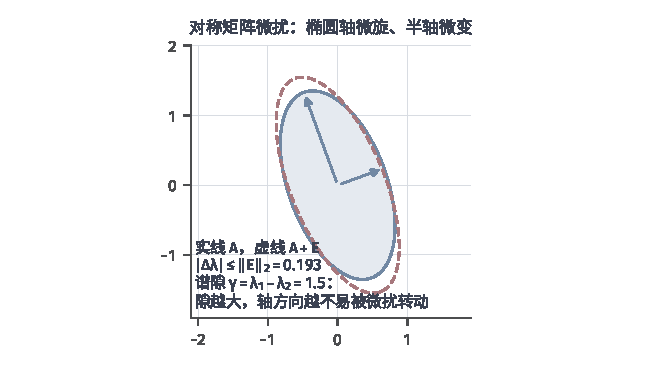
\includegraphics[width=112mm]{figures/00-shared/mathematical-preliminaries-upper/02-linear-spaces/matplotlib/ls-perturbation-ellipse/ls-perturbation-ellipse.pdf}
 \caption{对称矩阵微扰的谱与方向。实线椭圆$\bm x^\top\bm A\bm x=1$对应$\bm A$（特征值$2$与$0.5$，主轴
 方向$20^\circ$），虚线对应$\bm A+\bm E$（$\lVert\bm E\rVert_2\approx0.193$）：轴
 微旋、半轴微变。新特征值约$2.18$与$0.37$，偏移$0.18$、$0.13$均小于
 $\lVert\bm E\rVert_2$，符合Weyl界；未扰动的谱隙$\delta=\lambda_1-\lambda_2=1.5$越大，
 特征方向越不易被微扰转动。}
 \label{fig:ls-perturbation-ellipse}
\end{figure}

\paragraph{有序特征值的极值表征}

第~\ref{sec:ls-rayleigh-extremal}节的瑞利商$R_{\bm S}(\bm x)$（定义~\ref{def:matrix-analysis-rayleigh-quotient}）在整个空间上取最大、最小值。中间的特征值不再是整个空间上的极值，但可以先把方向限制在一个子空间内，再让子空间变动。第一步是说明受限的极值确实取到，并把它化成一个较小的对称矩阵的普通瑞利商问题。

\begin{lemma}[子空间上的瑞利商极值]
\label{lem:ls-restricted-rayleigh}
设$\bm S\in\mathbb R^{d\times d}$实对称，$\mathcal V$是$k$维子空间（$1\leq k\leq d$），$\bm U\in\mathbb R^{d\times k}$的列是$\mathcal V$的一组标准正交基。则对任意$\bm y\in\mathbb R^k\setminus\{\bm0\}$，
\[
 R_{\bm S}(\bm U\bm y)=R_{\bm U^\top\bm S\bm U}(\bm y).
\]
因而$R_{\bm S}$在$\mathcal V\setminus\{\bm0\}$上的最大值和最小值都取到，分别等于$k$阶实对称矩阵$\bm U^\top\bm S\bm U$的最大和最小特征值。
\end{lemma}
\begin{proof}
由$\bm U^\top\bm U=\bm I$，$(\bm U\bm y)^\top(\bm U\bm y)=\bm y^\top\bm y$，而$(\bm U\bm y)^\top\bm S(\bm U\bm y)=\bm y^\top(\bm U^\top\bm S\bm U)\bm y$，两式相除即得等式。$\bm U$的列线性无关，所以$\bm y\mapsto\bm U\bm y$是$\mathbb R^k\setminus\{\bm0\}$到$\mathcal V\setminus\{\bm0\}$的一一对应，$R_{\bm S}$在$\mathcal V\setminus\{\bm0\}$上的取值集合与$R_{\bm U^\top\bm S\bm U}$在$\mathbb R^k\setminus\{\bm0\}$上的取值集合相同。$\bm U^\top\bm S\bm U$实对称，由定理~\ref{thm:matrix-analysis-rayleigh-ritz}，后者的最大、最小值取到，且等于它的最大、最小特征值。
\end{proof}
矩阵$\bm U^\top\bm S\bm U$记录了$\bm S$在$\mathcal V$内部的二次型，可以看作$\bm S$在这个子空间上的压缩。引理把两件事分开：选哪个子空间是一回事，在选定的子空间内比较方向是另一回事，后者已由普通瑞利商的极值解决。受限极值是$R_{\bm S}$在$\mathcal V$上的取值，所以与基矩阵$\bm U$的选取无关。

有了受限极值，就可以让子空间变动：先在一个$k$维子空间上取瑞利商的最小值，再在所有$k$维子空间中取这些最小值的最大者。

\begin{theorem}[Courant--Fischer]
\label{thm:matrix-analysis-courant-fischer}
\label{eq:matrix-analysis-courant-fischer}
设$\bm S\in\mathbb R^{d\times d}$实对称，特征值为$\lambda_1\geq\cdots\geq\lambda_d$。对$k=1,\ldots,d$，
\begin{equation*}
\begin{aligned}
 \lambda_k
 &=\max_{\dim\mathcal V=k}\ \min_{\bm x\in\mathcal V,\bm x\neq\bm0}R_{\bm S}(\bm x)\\
 &=\min_{\dim\mathcal W=d-k+1}\ \max_{\bm x\in\mathcal W,\bm x\neq\bm0}R_{\bm S}(\bm x).
\end{aligned}
\end{equation*}
\end{theorem}
\begin{proof}
设$\bm q_1,\ldots,\bm q_d$是对应的标准正交特征向量。对单位向量$\bm x=\sum_ic_i\bm q_i$，有$R_{\bm S}(\bm x)=\sum_i\lambda_ic_i^2$，它是各特征值以$c_i^2$为权的加权平均。由引理~\ref{lem:ls-restricted-rayleigh}，每个子空间上的内层最小值与最大值都取到。

先证第一式。取$\mathcal V_k=\operatorname{span}\{\bm q_1,\ldots,\bm q_k\}$，其中单位向量的瑞利商是$\lambda_1,\ldots,\lambda_k$的加权平均，不小于$\lambda_k$；取$\bm x=\bm q_k$时等于$\lambda_k$。所以$\mathcal V_k$上的最小值为$\lambda_k$，外层的最大值至少为$\lambda_k$。反过来，任取$k$维子空间$\mathcal V$，令$\mathcal W_k=\operatorname{span}\{\bm q_k,\ldots,\bm q_d\}$，它是$d-k+1$维的。由维数公式，
\[
 \dim(\mathcal V\cap\mathcal W_k)\geq\dim\mathcal V+\dim\mathcal W_k-d=1,
\]
所以$\mathcal V$中有非零向量$\bm x$落在$\mathcal W_k$里。它的瑞利商是$\lambda_k,\ldots,\lambda_d$的加权平均，不大于$\lambda_k$，因此$\mathcal V$上瑞利商的最小值不超过$\lambda_k$。两方面合起来，外层最大值等于$\lambda_k$，并在$\mathcal V_k$处取到。

第二式交换两组特征向量的角色：$\mathcal W_k$上瑞利商的最大值恰为$\lambda_k$；任一$d-k+1$维子空间$\mathcal W$与$\mathcal V_k$的维数之和为$d+1$，二者有非零公共向量，其瑞利商不小于$\lambda_k$，所以$\mathcal W$上的最大值不小于$\lambda_k$。
\end{proof}
这一定理称为\term{最小最大原理}（min-max principle）。它只涉及子空间与瑞利商，不要求先知道特征向量，所以比较两个对称矩阵的同序特征值时，只需比较它们的瑞利商。第~\ref{sec:ls-low-rank-approximation}节的迹极值（定理~\ref{thm:matrix-analysis-trace-minimum}）也在$k$维子空间上取极值，但它汇总$k$个正交方向的贡献，刻画的是前$k$个特征值之和；最小最大原理刻画的是单个有序特征值。逐个比较特征值时需要后者。

\paragraph{谱值区间与正定性保证}

扰动对同一方向上瑞利商的影响很容易估计：由Cauchy--Schwarz不等式，对任意$\bm x$，
\[
 |\bm x^\top\bm E\bm x|\leq\lVert\bm x\rVert_2\lVert\bm E\bm x\rVert_2\leq\lVert\bm E\rVert_2\lVert\bm x\rVert_2^2 .
\]
最小最大原理把每个特征值写成瑞利商的受限极值，这一估计便逐层传到每个有序特征值上。

\begin{theorem}[Weyl特征值扰动界]
\label{thm:ls-weyl-eigenvalue}
设$\bm S,\bm E\in\mathbb R^{d\times d}$实对称。对每个$k=1,\ldots,d$，按降序配对的特征值满足
\begin{equation}
 |\lambda_k(\bm S+\bm E)-\lambda_k(\bm S)|\leq\lVert\bm E\rVert_2 .
 \label{eq:matrix-analysis-weyl-eigenvalue-perturbation}
\end{equation}
\end{theorem}
\begin{proof}
记$c=\lVert\bm E\rVert_2$。由上面的估计，对任意$\bm x\neq\bm0$，
\[
 R_{\bm S}(\bm x)-c\leq R_{\bm S+\bm E}(\bm x)\leq R_{\bm S}(\bm x)+c .
\]
任取$k$维子空间$\mathcal V$，由引理~\ref{lem:ls-restricted-rayleigh}，取$\bm x_*\in\mathcal V$使$R_{\bm S+\bm E}$在$\mathcal V$上达到最小，则
\[
 \begin{aligned}
 \min_{\mathcal V}R_{\bm S+\bm E}
 &=R_{\bm S+\bm E}(\bm x_*)\\
 &\geq R_{\bm S}(\bm x_*)-c\geq\min_{\mathcal V}R_{\bm S}-c ,
 \end{aligned}
\]
其中$\min_{\mathcal V}$表示在$\mathcal V\setminus\{\bm0\}$上取最小值。同理，取$R_{\bm S}$在$\mathcal V$上的最小点，得$\min_{\mathcal V}R_{\bm S+\bm E}\leq\min_{\mathcal V}R_{\bm S}+c$。这两个不等式对每个$k$维子空间都成立，对$\mathcal V$取最大值，由定理~\ref{thm:matrix-analysis-courant-fischer}即得$\lambda_k(\bm S)-c\leq\lambda_k(\bm S+\bm E)\leq\lambda_k(\bm S)+c$。
\end{proof}
因此，若$\lVert\bm E\rVert_2\leq\varepsilon$，每个真实特征值都落在区间$[\lambda_k(\bm S)-\varepsilon,\lambda_k(\bm S)+\varepsilon]$内。这个绝对误差界不要求特征值彼此分开，单重与重复特征值都适用。但它是绝对误差界：特征值本身接近零时，区间宽度$2\varepsilon$可能与特征值同量级，不能据此宣称相对误差也小。

区间立刻给出特征值符号的判断。若区间不含零，符号由区间确定；若区间含零，当前的误差预算不足以判断符号。例如$\bm S=\operatorname{diag}(1,\varepsilon/2)$，$0<\varepsilon<1$：取$\bm E=\bm0$时第二个特征值为正，取$\bm E=-\varepsilon\bm e_2\bm e_2^\top$时它变为$-\varepsilon/2$，两种扰动都满足预算。正定矩阵沿一条线段变化时，还可以得到对整条线段一致的下界。
\begin{theorem}[特征值的符号与正定性保持]
\label{thm:ls-eigenvalue-sign-definiteness}
设$\bm S,\bm E\in\mathbb R^{d\times d}$实对称，$\lVert\bm E\rVert_2\leq\varepsilon$。
\begin{enumerate}
 \item 若$\lambda_k(\bm S)>\varepsilon$，则$\lambda_k(\bm S+\bm E)>0$；若$\lambda_k(\bm S)<-\varepsilon$，则$\lambda_k(\bm S+\bm E)<0$。
 \item 若$\bm S$正定且$\varepsilon<\lambda_{\min}(\bm S)$，则对一切$t\in[0,1]$，
 \[
  \lambda_{\min}(\bm S+t\bm E)\geq\lambda_{\min}(\bm S)-\varepsilon>0 ,
 \]
 从而线段$\{\bm S+t\bm E:0\leq t\leq1\}$上的矩阵都正定。
\end{enumerate}
\end{theorem}
\begin{proof}
第1条：由定理~\ref{thm:ls-weyl-eigenvalue}，$\lambda_k(\bm S+\bm E)\geq\lambda_k(\bm S)-\varepsilon>0$；负号情形同理，$\lambda_k(\bm S+\bm E)\leq\lambda_k(\bm S)+\varepsilon<0$。第2条：对$t\in[0,1]$，$t\bm E$对称且$\lVert t\bm E\rVert_2=t\lVert\bm E\rVert_2\leq\varepsilon$。对最小特征值$\lambda_d$应用定理~\ref{thm:ls-weyl-eigenvalue}，得$\lambda_{\min}(\bm S+t\bm E)\geq\lambda_{\min}(\bm S)-\varepsilon>0$。实对称矩阵的特征值全为正时，由二次型展开式~\eqref{eq:matrix-analysis-quadratic-spectral-form}，它是正定的。
\end{proof}
第2条的下界$\lambda_{\min}(\bm S)-\varepsilon$与$t$无关。后文对正定矩阵求逆、开方或取对数时，常需确认整条线段都留在这些运算的定义域内，并且离定义域边界有一致的距离，例如第~\ref{sec:multivariable-logdet-differential}节估计对数行列式的变化；这个下界正好提供这一保证。

最后用一个例子检查界的精确程度，并看到有限变化界与可微性是两回事。
\begin{example}[重根处的最大特征值]
\label{ex:ls-weyl-double-root}
取$\bm S(t)=\operatorname{diag}(t,-t)$，$t\in\mathbb R$。$\bm S(0)=\bm0$的特征值$0$是二重根，而$\bm S(t)$的最大特征值为$|t|$。它相对于$\bm S(0)$的变化是$|t|$，恰好等于$\lVert\bm S(t)-\bm S(0)\rVert_2=|t|$，所以界~\eqref{eq:matrix-analysis-weyl-eigenvalue-perturbation}取等号。可见重根并不妨碍有限的绝对误差界。另一方面，$|t|$在$t=0$处左导数为$-1$、右导数为$1$，排序后的最大特征值在这里没有双侧导数。
\end{example}
第~\ref{sec:multivariable-local-condition-number}节再用这个例子区分有限敏感性与可微性；第~\ref{sec:multivariable-eigen-differential}节在特征值简单的条件下，另行研究所选分支的一阶响应。

\subsection{奇异值的扰动与秩判断}
\label{sec:ls-singular-value-sensitivity}

秩、可逆性与最佳低秩逼近的误差都由奇异值决定。本小节先把上一小节的特征值区间移到奇异值上，再据此判断哪些关于秩的结论在误差预算下仍然可靠。

\paragraph{奇异值的误差区间}

长方矩阵没有特征值，不能直接使用Weyl界。办法是把它放进一个对称矩阵，使后者的特征值恰好包含原矩阵的奇异值。对$\bm A\in\mathbb R^{m\times n}$，记$p=\min(m,n)$，奇异值为$\sigma_1(\bm A)\geq\cdots\geq\sigma_p(\bm A)\geq0$，定义$(m+n)$阶对称增广矩阵
\[
 \bm H(\bm A)=\begin{bmatrix}\bm0&\bm A\\\bm A^\top&\bm0\end{bmatrix},
\]

\begin{lemma}[对称增广矩阵的谱]
\label{lem:ls-symmetric-augmentation-spectrum}
$\bm H(\bm A)$的特征值为$\pm\sigma_1(\bm A)$、$\ldots$、$\pm\sigma_p(\bm A)$，以及$|m-n|$个零。特别地，按降序排列时它的前$p$个特征值依次为$\sigma_1(\bm A),\ldots,\sigma_p(\bm A)$；并且$\lVert\bm H(\bm A)\rVert_2=\lVert\bm A\rVert_2$。
\end{lemma}
\begin{proof}
由定理~\ref{thm:ls-svd-existence}，取完整的SVD $\bm A=\bm U\bm\Sigma\bm V^\top$，列向量为$\bm u_1,\ldots,\bm u_m$与$\bm v_1,\ldots,\bm v_n$。对$i\leq p$，有$\bm A\bm v_i=\sigma_i\bm u_i$与$\bm A^\top\bm u_i=\bm V\bm\Sigma^\top\bm e_i=\sigma_i\bm v_i$。令
\[
 \bm w_i^{\pm}=\frac1{\sqrt2}\begin{bmatrix}\bm u_i\\\pm\bm v_i\end{bmatrix},
\]
用$(\bm a;\bm b)$表示把$\bm a$、$\bm b$上下拼接成的列向量，则
\[
 \bm H(\bm A)\bm w_i^{\pm}=\tfrac1{\sqrt2}(\pm\bm A\bm v_i;\bm A^\top\bm u_i)=\tfrac1{\sqrt2}(\pm\sigma_i\bm u_i;\sigma_i\bm v_i)=\pm\sigma_i\bm w_i^{\pm}.
\]
若$m>n$，对$j>n$，$\bm\Sigma^\top$的第$j$列为零，故$\bm A^\top\bm u_j=\bm0$，向量$(\bm u_j;\bm0)$是特征值$0$的特征向量；若$n>m$，对$j>m$有$\bm A\bm v_j=\bm0$，向量$(\bm0;\bm v_j)$是特征值$0$的特征向量。这$2p+|m-n|=m+n$个向量两两正交且长度为$1$：由$\bm u_i$、$\bm v_i$各自标准正交，$\bm w_i^{\pm}$与$\bm w_j^{\pm}$的内积为$\tfrac12(\bm u_i^\top\bm u_j\pm\bm v_i^\top\bm v_j)$，两者符号相同时取正号、相反时取负号，所以$i\neq j$时为零，$i=j$而符号相反时为$\tfrac12(1-1)=0$，符号相同时为$1$；补充的向量$(\bm u_j;\bm0)$或$(\bm0;\bm v_j)$只含$j>p$的分量，与所有$\bm w_i^{\pm}$及彼此都正交。所以它们构成$\bm H(\bm A)$的标准正交特征基，列出了全部特征值（计重数）。$\sigma_i\geq0\geq-\sigma_j$，所以降序排列时前$p$个是$\sigma_1,\ldots,\sigma_p$。

最后，对$\bm z=(\bm y;\bm x)$，$\bm H(\bm A)\bm z=(\bm A\bm x;\bm A^\top\bm y)$。$\bm A^\top$与$\bm A$有相同的非零奇异值，所以$\lVert\bm A^\top\rVert_2=\lVert\bm A\rVert_2$，于是
\[
 \begin{aligned}
 \lVert\bm H(\bm A)\bm z\rVert_2^2
 &=\lVert\bm A\bm x\rVert_2^2+\lVert\bm A^\top\bm y\rVert_2^2\\
 &\leq\lVert\bm A\rVert_2^2\bigl(\lVert\bm x\rVert_2^2+\lVert\bm y\rVert_2^2\bigr)
 =\lVert\bm A\rVert_2^2\lVert\bm z\rVert_2^2 ,
 \end{aligned}
\]
而$\bm z=\bm w_1^+$时$\lVert\bm H(\bm A)\bm z\rVert_2=\sigma_1=\lVert\bm A\rVert_2$，故$\lVert\bm H(\bm A)\rVert_2=\lVert\bm A\rVert_2$。
\end{proof}

\begin{theorem}[奇异值的Weyl界]
\label{thm:ls-weyl-singular-value}
设$\bm A,\bm E\in\mathbb R^{m\times n}$，$p=\min(m,n)$。对$i=1,\ldots,p$，
\begin{equation}
 |\sigma_i(\bm A+\bm E)-\sigma_i(\bm A)|\leq\lVert\bm E\rVert_2 .
 \label{eq:matrix-analysis-singular-value-perturbation}
\end{equation}
\end{theorem}
\begin{proof}
增广是线性的：$\bm H(\bm A+\bm E)=\bm H(\bm A)+\bm H(\bm E)$，三者都实对称。对$\bm H(\bm A)$与扰动$\bm H(\bm E)$应用定理~\ref{thm:ls-weyl-eigenvalue}，第$i$个特征值的变化不超过$\lVert\bm H(\bm E)\rVert_2$。由引理~\ref{lem:ls-symmetric-augmentation-spectrum}，$i\leq p$时第$i$个特征值就是第$i$个奇异值，且$\lVert\bm H(\bm E)\rVert_2=\lVert\bm E\rVert_2$。
\end{proof}
奇异值非负，所以在误差预算$\lVert\bm E\rVert_2\leq\varepsilon$下，真实的第$i$个奇异值落在非负区间$[\max(0,\sigma_i(\bm A)-\varepsilon),\ \sigma_i(\bm A)+\varepsilon]$内。

最佳低秩逼近的误差也随之受控。由定理~\ref{thm:matrix-analysis-best-low-rank}，对$0\leq k<p$，秩不超过$k$的矩阵中，与$\bm A$的最小谱范数距离为$\sigma_{k+1}(\bm A)$。把定理~\ref{thm:ls-weyl-singular-value}用于$i=k+1$，扰动前后这个最优误差之差不超过$\varepsilon$。要注意，这只说明最优误差的数值稳定；取得最优误差的低秩矩阵及其所用的奇异方向是否同样稳定，是另一个问题，留到下一小节。

\paragraph{秩保证与可逆性的边界}

奇异值区间不含零，就能保证相应的奇异值为正，从而给出秩的下界。
\begin{theorem}[由奇异值保证秩]
\label{thm:ls-singular-value-rank-guarantee}
设$\bm A,\bm E\in\mathbb R^{m\times n}$，$\lVert\bm E\rVert_2\leq\varepsilon$，$1\leq k\leq\min(m,n)$。若$\sigma_k(\bm A)>\varepsilon$，则$\operatorname{rank}(\bm A+\bm E)\geq k$。特别地，$m\geq n$且$\sigma_n(\bm A)>\varepsilon$时，$\bm A+\bm E$满列秩。
\end{theorem}
\begin{proof}
由定理~\ref{thm:ls-weyl-singular-value}，$\sigma_k(\bm A+\bm E)\geq\sigma_k(\bm A)-\varepsilon>0$，而奇异值降序排列，所以$\bm A+\bm E$至少有$k$个正奇异值。由定理~\ref{thm:ls-svd-existence}，正奇异值的个数等于秩。
\end{proof}
反方向的结论不成立：$\sigma_k(\bm A)\leq\varepsilon$只表示区间$[\max(0,\sigma_k(\bm A)-\varepsilon),\sigma_k(\bm A)+\varepsilon]$包含零，无法排除真实矩阵的第$k$个奇异值为零，但也不能由此断言真实矩阵秩亏。本小节只给出由误差预算能够保证的结论；实际计算中怎样选取阈值、把大于阈值的奇异值个数作为数值秩，在第~\ref{sec:ls-pseudoinverse-rank-change}节结合求解任务讨论。

对可逆方阵，同样的想法回答：最小要多大的扰动，才能使它变成奇异矩阵？
\begin{theorem}[到奇异矩阵的距离]
\label{thm:ls-distance-to-singularity}
设$\bm A\in\mathbb R^{n\times n}$可逆，奇异值为$\sigma_1\geq\cdots\geq\sigma_n>0$，$\bm u_n$、$\bm v_n$是与$\sigma_n$对应的单位左、右奇异向量。则
\[
 \min\{\lVert\bm E\rVert_2:\bm A+\bm E\text{ 奇异}\}=\sigma_n(\bm A),
\]
最小值在$\bm E_*=-\sigma_n\bm u_n\bm v_n^\top$处取到。相对于$\lVert\bm A\rVert_2$，这个距离为
\[
 \frac{\sigma_n(\bm A)}{\lVert\bm A\rVert_2}=\frac1{\kappa_2(\bm A)} .
\]
\end{theorem}
\begin{proof}
$n$阶方阵奇异，当且仅当它的秩不超过$n-1$。由定理~\ref{thm:matrix-analysis-best-low-rank}，秩不超过$n-1$的矩阵$\bm B$与$\bm A$的最小谱范数距离为$\sigma_n$，令$\bm E=\bm B-\bm A$即得结论。下面再给出不依赖该定理的直接验证。

下界：设$\lVert\bm E\rVert_2<\sigma_n$。对任意$\bm x\neq\bm0$，由定理~\ref{thm:matrix-analysis-condition-number-bound}证明中的估计$\lVert\bm A\bm x\rVert_2\geq\sigma_n\lVert\bm x\rVert_2$，
\[
 \begin{aligned}
 \lVert(\bm A+\bm E)\bm x\rVert_2
 &\geq\lVert\bm A\bm x\rVert_2-\lVert\bm E\bm x\rVert_2\\
 &\geq(\sigma_n-\lVert\bm E\rVert_2)\lVert\bm x\rVert_2>0 ,
 \end{aligned}
\]
所以$\bm A+\bm E$的零空间只含零向量，它可逆。可达：对任意$\bm x$，$\lVert\bm u_n\bm v_n^\top\bm x\rVert_2=|\bm v_n^\top\bm x|\leq\lVert\bm x\rVert_2$，且$\bm x=\bm v_n$时取等号，故$\lVert\bm E_*\rVert_2=\sigma_n$；又$(\bm A+\bm E_*)\bm v_n=\sigma_n\bm u_n-\sigma_n\bm u_n=\bm0$，所以$\bm A+\bm E_*$奇异。相对距离由$\lVert\bm A\rVert_2=\sigma_1$与$\kappa_2(\bm A)=\sigma_1/\sigma_n$得到。
\end{proof}
这为上一节的矩阵条件数提供了另一种解释：$\kappa_2(\bm A)$越大，按相对尺度计，$\bm A$离奇异矩阵越近。这个结论的条件是允许任意的谱范数扰动；若扰动必须保持某种结构，例如对称或稀疏，可选的扰动变少，本定理只给出距离的下界，相应的距离需要另行分析。还要注意，扰动超过$\sigma_n$并不意味着每个这样的扰动都使矩阵奇异，例如$\bm E=\bm A$的范数为$\sigma_1\geq\sigma_n$，而$\bm A+\bm E=2\bm A$仍然可逆。

\begin{example}[对角矩阵的可逆性边界]
\label{ex:ls-diagonal-distance-to-singularity}
取$\bm A=\operatorname{diag}(1,s)$，$0<s<1$。它的奇异值为$1$与$s$，$\kappa_2(\bm A)=1/s$。由定理~\ref{thm:ls-distance-to-singularity}，误差预算$\varepsilon<s$时可以保证$\bm A+\bm E$可逆；而$\bm E=-s\bm e_2\bm e_2^\top$的范数恰为$s$，它把$\bm A$变成奇异的$\operatorname{diag}(1,0)$。相对距离$s/1=1/\kappa_2(\bm A)$。
\end{example}
在这个例子中，$s$很小时矩阵离奇异很近，但它的第一奇异方向$\bm e_1$并不因此变得不稳定。下一小节将说明，保留第一奇异方向的稳定性由截断处的间隙$\sigma_1-\sigma_2=1-s$决定，而可逆性的边界由最小奇异值$s$决定，二者不能互相替代。

\subsection{特征子空间的扰动}
\label{sec:ls-subspace-sensitivity}

即使特征值的绝对误差很小，按这些特征值选出的方向也可能变化很大。本小节研究：在给定的误差预算下，原来选出的特征子空间能偏转多少。先建立一种不依赖基的选择的子空间距离，再检查目标特征值组与其余特征值之间的间隔。

\paragraph{子空间的距离}

比较特征向量时，比较对象应是子空间本身。特征向量可以变号；特征值重复时，特征空间内部还可以任意换标准正交基，这些都不改变子空间，所以单个基向量的变化不能当作子空间的误差。图~\ref{fig:ls-principal-angles-subspaces}从两条过原点的直线看起：两直线的夹角与方向向量的选取无关；把一条直线的单位方向向量投影到另一条上，投影不掉的部分长度为$\sin\theta$。

\begin{figure}[htbp]
 \centering
 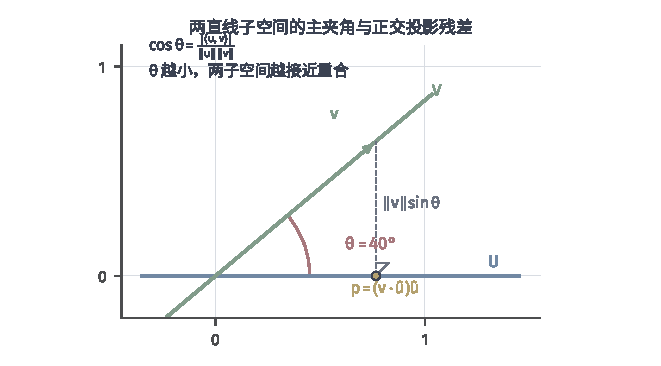
\includegraphics[width=112mm]{figures/00-shared/mathematical-preliminaries-upper/02-linear-spaces/matplotlib/ls-principal-angles-subspaces/ls-principal-angles-subspaces.pdf}
 \caption{两条直线子空间的主夹角。蓝线为$\bm U$、绿线为$\bm V$，红弧为主夹角
 $\theta=40^\circ$；黄点$\bm p$是$\bm v$在$\bm U$上的正交投影，灰虚线为投影
 垂线。$\cos40^\circ\approx0.766$、$\sin40^\circ\approx0.643$，残差长度
 $\lVert\bm v\rVert\sin\theta$即投影不掉的分量。}
 \label{fig:ls-principal-angles-subspaces}
\end{figure}

对一维子空间，若$\bm q,\widetilde{\bm q}$是单位方向向量，则$|\bm q^\top\widetilde{\bm q}|=\cos\theta$。高维子空间之间有多个夹角，由交叉内积矩阵的奇异值给出。
\begin{definition}[主夹角]
\label{def:matrix-analysis-principal-angles}
设$\bm Q,\widetilde{\bm Q}\in\mathbb R^{d\times r}$列标准正交，分别张成$r$维子空间。交叉矩阵$\bm Q^\top\widetilde{\bm Q}$的奇异值记为$\cos\theta_1\geq\dots\geq\cos\theta_r$，$0\leq\theta_1\leq\cdots\leq\theta_r\leq\pi/2$，这些$\theta_i$称为两个子空间的\term{主夹角}（principal angles）。
\end{definition}
这些奇异值都在$[0,1]$内，因为$\lVert\bm Q^\top\widetilde{\bm Q}\rVert_2\leq\lVert\bm Q\rVert_2\lVert\widetilde{\bm Q}\rVert_2=1$，所以$\theta_i$有定义。换基相当于把$\bm Q$、$\widetilde{\bm Q}$分别右乘$r$阶正交矩阵$\bm R$、$\widetilde{\bm R}$，交叉矩阵变为$\bm R^\top(\bm Q^\top\widetilde{\bm Q})\widetilde{\bm R}$，奇异值不变，所以主夹角只依赖两个子空间。最大主夹角$\theta_r$记为$\theta_{\max}$。

主夹角的正弦度量一个子空间伸出另一个子空间的部分，它们也可以直接读出，并与正交投影之差联系起来。设$\widetilde{\bm Q}_\perp\in\mathbb R^{d\times(d-r)}$的列是$\widetilde{\bm Q}$列空间正交补的标准正交基，记
\[
 \bm C=\widetilde{\bm Q}^\top\bm Q,\qquad\bm X=\widetilde{\bm Q}_\perp^\top\bm Q ,
\]
再记两个子空间上的正交投影为$\bm P=\bm Q\bm Q^\top$、$\widetilde{\bm P}=\widetilde{\bm Q}\widetilde{\bm Q}^\top$，它们与基的选取无关。
\begin{theorem}[主夹角的正弦与投影之差]
\label{thm:ls-principal-angle-projection}
在上述记号下，$\bm X^\top\bm X=\bm I-\bm C^\top\bm C$，其特征值为$\sin^2\theta_1,\ldots,\sin^2\theta_r$，并且
\[
 \tfrac12\lVert\bm P-\widetilde{\bm P}\rVert_{\mathrm F}^2=\sum_{i=1}^r\sin^2\theta_i=\lVert\bm X\rVert_{\mathrm F}^2 .
\]
\end{theorem}
\begin{proof}
$[\widetilde{\bm Q},\widetilde{\bm Q}_\perp]$是正交矩阵，所以对任意$\bm a\in\mathbb R^r$，把$\bm Q\bm a$分解到$\widetilde{\bm Q}$的列空间与其正交补，由勾股定理，
\[
 \lVert\bm C\bm a\rVert_2^2+\lVert\bm X\bm a\rVert_2^2=\lVert\bm Q\bm a\rVert_2^2=\lVert\bm a\rVert_2^2 .
\]
即对称矩阵$\bm X^\top\bm X$与$\bm I-\bm C^\top\bm C$的二次型处处相等。对称矩阵由其二次型唯一确定（用$\bm a+\bm b$与$\bm a-\bm b$的二次型之差可以读出$\bm a^\top\bm M\bm b$），所以$\bm X^\top\bm X=\bm I-\bm C^\top\bm C$。$\bm C$是交叉矩阵$\bm Q^\top\widetilde{\bm Q}$的转置，$\bm C^\top\bm C$的特征值是$\cos^2\theta_i$，所以$\bm X^\top\bm X$的特征值是$1-\cos^2\theta_i=\sin^2\theta_i$，且$\lVert\bm X\rVert_{\mathrm F}^2=\operatorname{tr}(\bm X^\top\bm X)=\sum_i\sin^2\theta_i$。

再算投影之差。$\bm P$、$\widetilde{\bm P}$对称且$\bm P^2=\bm P$、$\widetilde{\bm P}^2=\widetilde{\bm P}$，$\operatorname{tr}\bm P=\operatorname{tr}(\bm Q^\top\bm Q)=r$，同样$\operatorname{tr}\widetilde{\bm P}=r$。于是
\[
 \begin{aligned}
 \lVert\bm P-\widetilde{\bm P}\rVert_{\mathrm F}^2
 &=\operatorname{tr}\bigl((\bm P-\widetilde{\bm P})^2\bigr)\\
 &=\operatorname{tr}\bm P-2\operatorname{tr}(\bm P\widetilde{\bm P})+\operatorname{tr}\widetilde{\bm P}\\
 &=2r-2\operatorname{tr}(\bm P\widetilde{\bm P}).
 \end{aligned}
\]
由迹的循环性，$\operatorname{tr}(\bm P\widetilde{\bm P})=\operatorname{tr}(\widetilde{\bm Q}^\top\bm Q\bm Q^\top\widetilde{\bm Q})=\lVert\bm Q^\top\widetilde{\bm Q}\rVert_{\mathrm F}^2=\sum_i\cos^2\theta_i$，代入得$\lVert\bm P-\widetilde{\bm P}\rVert_{\mathrm F}^2=2\sum_i(1-\cos^2\theta_i)=2\sum_i\sin^2\theta_i$。
\end{proof}
Frobenius范数汇总了所有主夹角，反映整体偏转。只关心最坏的那个方向时，用谱范数，它恰好读出最大主夹角。
\begin{theorem}[投影之差的谱范数]
\label{thm:ls-projection-spectral-distance}
在定理~\ref{thm:ls-principal-angle-projection}的记号下，
\[
 \lVert\bm P-\widetilde{\bm P}\rVert_2=\lVert\bm X\rVert_2=\sin\theta_{\max}.
\]
\end{theorem}
\begin{proof}
由定理~\ref{thm:ls-principal-angle-projection}，$\bm X^\top\bm X$的最大特征值是$\sin^2\theta_{\max}$，所以$\lVert\bm X\rVert_2=\sin\theta_{\max}$。

再设$\bm Q_\perp\in\mathbb R^{d\times(d-r)}$的列是$\bm Q$列空间正交补的标准正交基，于是$\bm I-\bm P=\bm Q_\perp\bm Q_\perp^\top$、$\bm I-\widetilde{\bm P}=\widetilde{\bm Q}_\perp\widetilde{\bm Q}_\perp^\top$。先说明两个算子范数。列标准正交的矩阵保持长度，行标准正交的矩阵不增加长度，并在其行空间上保持长度，所以
\[
 \lVert(\bm I-\widetilde{\bm P})\bm P\rVert_2
 =\lVert\widetilde{\bm Q}_\perp(\widetilde{\bm Q}_\perp^\top\bm Q)\bm Q^\top\rVert_2
 =\lVert\bm X\rVert_2 .
\]
同理$\lVert(\bm I-\bm P)\widetilde{\bm P}\rVert_2=\lVert\bm Q_\perp^\top\widetilde{\bm Q}\rVert_2$。把定理~\ref{thm:ls-principal-angle-projection}中两个子空间的角色交换，交叉矩阵变为$\widetilde{\bm Q}^\top\bm Q$，它与原交叉矩阵互为转置，奇异值相同，所以$\bm Q_\perp^\top\widetilde{\bm Q}$的最大奇异值同样是$\sin\theta_{\max}$。

上界：直接展开可验证
\[
 \bm P-\widetilde{\bm P}=\bm P(\bm I-\widetilde{\bm P})-(\bm I-\bm P)\widetilde{\bm P}.
\]
对任意$\bm z$，右端第一项落在$\bm Q$的列空间中，第二项落在其正交补中，由勾股定理，
\[
 \begin{aligned}
 \lVert(\bm P-\widetilde{\bm P})\bm z\rVert_2^2
 &=\lVert\bm P(\bm I-\widetilde{\bm P})\bm z\rVert_2^2+\lVert(\bm I-\bm P)\widetilde{\bm P}\bm z\rVert_2^2\\
 &\leq\sin^2\theta_{\max}\bigl(\lVert(\bm I-\widetilde{\bm P})\bm z\rVert_2^2+\lVert\widetilde{\bm P}\bm z\rVert_2^2\bigr)\\
 &=\sin^2\theta_{\max}\lVert\bm z\rVert_2^2 .
 \end{aligned}
\]
这里第二行用到$\bm P(\bm I-\widetilde{\bm P})=\bigl((\bm I-\widetilde{\bm P})\bm P\bigr)^\top$，转置不改变谱范数，并对两项分别使用上面的范数等式；第三行再用勾股定理。

下界：取单位向量$\bm a\in\mathbb R^r$使$\lVert\bm X\bm a\rVert_2=\lVert\bm X\rVert_2$（取$\bm X$的第一右奇异向量），令$\bm z=\bm Q\bm a$，则$\lVert\bm z\rVert_2=1$，$\bm P\bm z=\bm z$，
\[
 (\bm P-\widetilde{\bm P})\bm z=(\bm I-\widetilde{\bm P})\bm Q\bm a=\widetilde{\bm Q}_\perp\bm X\bm a ,
\]
长度为$\lVert\bm X\bm a\rVert_2=\sin\theta_{\max}$。两方面合起来即得结论。
\end{proof}

\paragraph{谱隙控制的偏转界}

现在比较特征子空间。设$\bm S$、$\widetilde{\bm S}=\bm S+\bm E\in\mathbb R^{d\times d}$实对称，取$1\leq k<d$，比较两者前$k$个特征值对应的子空间。要使比较有意义，原矩阵的目标特征值组必须与其余特征值分开：设截断处的\term{谱隙}（spectral gap）
\[
 \delta=\lambda_k(\bm S)-\lambda_{k+1}(\bm S)>0 ,
\]
这时$\bm S$前$k$个特征值对应的特征子空间是唯一确定的$k$维子空间。若误差预算满足$\lVert\bm E\rVert_2\leq\varepsilon<\delta/2$，由Weyl界，
\[
 \lambda_k(\widetilde{\bm S})\geq\lambda_k(\bm S)-\varepsilon>\lambda_{k+1}(\bm S)+\varepsilon\geq\lambda_{k+1}(\widetilde{\bm S}),
\]
扰动后截断处仍然严格分开，$\widetilde{\bm S}$前$k$个特征值的特征子空间也唯一确定，两者都是$k$维，可以用主夹角比较。下面的论证用到的是交叉谱间隔
\[
 \gamma=\lambda_k(\bm S)-\lambda_{k+1}(\widetilde{\bm S}),
\]
即原目标组的最小特征值与扰动后其余特征值的最大者之差。由Weyl界$\lambda_{k+1}(\widetilde{\bm S})\leq\lambda_{k+1}(\bm S)+\varepsilon$，得$\gamma\geq\delta-\varepsilon>0$。

记$\bm Q\in\mathbb R^{d\times k}$的列是$\bm S$前$k$个特征值的标准正交特征向量，$\bm\Lambda_1=\operatorname{diag}(\lambda_1(\bm S),\ldots,\lambda_k(\bm S))$；$\widetilde{\bm Q}$的列是$\widetilde{\bm S}$前$k$个特征值的标准正交特征向量，$\widetilde{\bm Q}_\perp$的列是其余的标准正交特征向量，对应特征值组成对角矩阵$\widetilde{\bm\Lambda}_2=\operatorname{diag}(\lambda_{k+1}(\widetilde{\bm S}),\ldots,\lambda_d(\widetilde{\bm S}))$。令$\bm X=\widetilde{\bm Q}_\perp^\top\bm Q$，由定理~\ref{thm:ls-principal-angle-projection}，它的Frobenius范数平方就是两个子空间主夹角正弦的平方和。

\begin{theorem}[特征子空间偏转的Frobenius界]
\label{thm:ls-gap-subspace-frobenius}
在上述记号下，若$\gamma=\lambda_k(\bm S)-\lambda_{k+1}(\widetilde{\bm S})>0$，则$\bm Q$与$\widetilde{\bm Q}$张成的子空间的主夹角$\theta_1,\ldots,\theta_k$满足
\[
 \begin{aligned}
 \Bigl(\sum_{i=1}^k\sin^2\theta_i\Bigr)^{1/2}
 &=\lVert\bm X\rVert_{\mathrm F}\\
 &\leq\frac{\lVert\widetilde{\bm Q}_\perp^\top\bm E\bm Q\rVert_{\mathrm F}}{\gamma}
 \leq\frac{\lVert\bm E\bm Q\rVert_{\mathrm F}}{\gamma}.
 \end{aligned}
\]
\end{theorem}
\begin{proof}
由特征关系$\widetilde{\bm Q}_\perp^\top\widetilde{\bm S}=\widetilde{\bm\Lambda}_2\widetilde{\bm Q}_\perp^\top$（对$\widetilde{\bm S}\widetilde{\bm Q}_\perp=\widetilde{\bm Q}_\perp\widetilde{\bm\Lambda}_2$取转置）右乘$\bm Q$，又由$\bm S\bm Q=\bm Q\bm\Lambda_1$左乘$\widetilde{\bm Q}_\perp^\top$，两式相减，并用$\widetilde{\bm S}-\bm S=\bm E$，得
\[
 \widetilde{\bm\Lambda}_2\bm X-\bm X\bm\Lambda_1=\widetilde{\bm Q}_\perp^\top\bm E\bm Q .
\]
这是关于$\bm X$的线性方程，两侧的系数矩阵都是对角的，可以逐元素读出。把$\bm X$的行用$j=k+1,\ldots,d$编号、列用$i=1,\ldots,k$编号，第$(j,i)$元满足
\[
 \bigl(\lambda_j(\widetilde{\bm S})-\lambda_i(\bm S)\bigr)X_{j,i}=(\widetilde{\bm Q}_\perp^\top\bm E\bm Q)_{j,i}.
\]
由降序，$i\leq k<j$时$\lambda_i(\bm S)-\lambda_j(\widetilde{\bm S})\geq\lambda_k(\bm S)-\lambda_{k+1}(\widetilde{\bm S})=\gamma>0$，所以$|X_{j,i}|\leq|(\widetilde{\bm Q}_\perp^\top\bm E\bm Q)_{j,i}|/\gamma$。逐元素平方求和，得第一个不等式。$\widetilde{\bm Q}_\perp^\top$的行标准正交，对任意向量$\bm m$有$\lVert\widetilde{\bm Q}_\perp^\top\bm m\rVert_2\leq\lVert\bm m\rVert_2$，按列应用于$\bm E\bm Q$即得第二个不等式。等式部分来自定理~\ref{thm:ls-principal-angle-projection}。
\end{proof}
证明中出现的方程同时含有左乘和右乘未知矩阵的两项，这类方程称为Sylvester方程，第~\ref{sec:ls-matrix-equations}节专门研究它；这里两侧系数都是对角矩阵，逐元素相除就够了。由$\lVert\bm E\bm Q\rVert_{\mathrm F}\leq\sqrt k\,\lVert\bm E\rVert_2$，右端不超过$\sqrt k\,\lVert\bm E\rVert_2/\gamma$。

对谱范数，即最大主夹角，也有同型的结论。它不是上面Frobenius估计的直接推论：由Frobenius界只能得到带因子$\sqrt k$的估计。去掉这个因子要换一种读法：不逐元素相除，而是用$\bm X$的最大奇异方向从两侧检验同一个矩阵方程。
\begin{theorem}[Davis--Kahan谱隙界]
\label{thm:ls-davis-kahan}
在定理~\ref{thm:ls-gap-subspace-frobenius}的条件下，
\begin{equation}
 \lVert\widetilde{\bm P}-\bm P\rVert_2=\sin\theta_{\max}
 \leq\frac{\lVert\bm E\bm Q\rVert_2}{\gamma}\leq\frac{\lVert\bm E\rVert_2}{\gamma}.
 \label{eq:matrix-analysis-eigenvector-gap-bound}
\end{equation}
\end{theorem}
\begin{proof}
由定理~\ref{thm:ls-projection-spectral-distance}，$\lVert\widetilde{\bm P}-\bm P\rVert_2=\sin\theta_{\max}=\lVert\bm X\rVert_2$，记$s=\lVert\bm X\rVert_2$。$s=0$时结论成立，下设$s>0$。取$\bm X$的第一右、左奇异向量$\bm a\in\mathbb R^k$、$\bm b\in\mathbb R^{d-k}$，它们是单位向量，满足$\bm X\bm a=s\bm b$、$\bm X^\top\bm b=s\bm a$。用$\bm b^\top$左乘、$\bm a$右乘定理~\ref{thm:ls-gap-subspace-frobenius}证明中的方程$\widetilde{\bm\Lambda}_2\bm X-\bm X\bm\Lambda_1=\widetilde{\bm Q}_\perp^\top\bm E\bm Q$，左端为
\[
 \begin{aligned}
 &\bm b^\top\widetilde{\bm\Lambda}_2(\bm X\bm a)-(\bm X^\top\bm b)^\top\bm\Lambda_1\bm a\\
 &\quad=s\bigl(\bm b^\top\widetilde{\bm\Lambda}_2\bm b-\bm a^\top\bm\Lambda_1\bm a\bigr).
 \end{aligned}
\]
$\bm\Lambda_1$的对角元都不小于$\lambda_k(\bm S)$，$\bm a$是单位向量，所以
\[
 \bm a^\top\bm\Lambda_1\bm a=\sum_i\lambda_i(\bm S)a_i^2\geq\lambda_k(\bm S);
\]
同理$\bm b^\top\widetilde{\bm\Lambda}_2\bm b\leq\lambda_{k+1}(\widetilde{\bm S})$。于是左端的绝对值至少为$s\gamma$。右端的绝对值满足
\[
 |\bm b^\top\widetilde{\bm Q}_\perp^\top\bm E\bm Q\bm a|
 \leq\lVert\widetilde{\bm Q}_\perp\bm b\rVert_2\,\lVert\bm E\bm Q\bm a\rVert_2
 \leq\lVert\bm E\bm Q\rVert_2 ,
\]
其中用到$\lVert\widetilde{\bm Q}_\perp\bm b\rVert_2=\lVert\bm b\rVert_2=1$。所以$s\gamma\leq\lVert\bm E\bm Q\rVert_2$，即第一个不等式。最后$\lVert\bm E\bm Q\bm a\rVert_2\leq\lVert\bm E\rVert_2\lVert\bm Q\bm a\rVert_2=\lVert\bm E\rVert_2$，得第二个不等式。
\end{proof}
这个证明只用到单侧的谱分离：原目标组的特征值都不小于$\lambda_k(\bm S)$，扰动后其余的特征值都不大于$\lambda_{k+1}(\widetilde{\bm S})$。这正是本节使用的情形；目标组位于谱的中间、两侧都有其余特征值时，需要另作处理，本节不使用。

把交叉间隔换成事先就能检查的量：若已知原谱隙$\delta$且$\lVert\bm E\rVert_2\leq\varepsilon<\delta/2$，前面已得$\gamma\geq\delta-\varepsilon$，于是
\[
 \lVert\widetilde{\bm P}-\bm P\rVert_2\leq\frac{\varepsilon}{\delta-\varepsilon}\leq\frac{2\varepsilon}{\delta},
\]
后一个不等号用到$\delta-\varepsilon>\delta/2$。谱隙在分母上：谱隙越小，同样的扰动能使子空间转过的角度越大。若已经知道交叉间隔$\gamma>0$，也可以直接使用带$\gamma$的形式；原谱隙与误差预算只是一组便于事先检查的充分条件。

下面的二维例子可以精确算出转角，并说明子空间的敏感程度不能由矩阵条件数判断。
\begin{example}[谱隙与特征方向的转角]
\label{ex:ls-gap-direction-rotation}
取$\bm S=\operatorname{diag}(1+\delta,1)$与交叉扰动
\[
 \bm E=t\begin{bmatrix}0&1\\1&0\end{bmatrix},\qquad\delta>0,\ t\geq0 .
\]
$\bm S$的谱隙为$\delta$，最大特征方向是$\bm e_1$，$\lVert\bm E\rVert_2=t$。把扰动后的矩阵写成单位矩阵的倍数加一个迹为零的部分：
\[
 \bm S+\bm E=\bigl(1+\tfrac\delta2\bigr)\bm I+\bm M,\qquad
 \bm M=\begin{bmatrix}\delta/2&t\\t&-\delta/2\end{bmatrix}.
\]
加上单位矩阵的倍数不改变特征向量。记$r=\sqrt{\delta^2/4+t^2}>0$，取$\theta\in[0,\pi/4)$满足$\cos2\theta=\delta/(2r)$、$\sin2\theta=t/r$，即
\[
 \tan2\theta=\frac{2t}{\delta}.
\]
于是$\bm M=r\left[\begin{smallmatrix}\cos2\theta&\sin2\theta\\\sin2\theta&-\cos2\theta\end{smallmatrix}\right]$，由两角差公式，
\[
 \bm M\begin{bmatrix}\cos\theta\\\sin\theta\end{bmatrix}
 =r\begin{bmatrix}\cos(2\theta-\theta)\\\sin(2\theta-\theta)\end{bmatrix}
 =r\begin{bmatrix}\cos\theta\\\sin\theta\end{bmatrix}.
\]
$\bm M$的迹为零，另一个特征值是$-r$。所以$\bm S+\bm E$的特征值为$1+\delta/2\pm r$，最大特征方向从$\bm e_1$转到$(\cos\theta,\sin\theta)^\top$，转角$\theta$满足$\tan2\theta=2t/\delta$。

$\bm S$的条件数$\kappa_2(\bm S)=1+\delta$，$\delta$小时接近$1$；但取$t=\delta/2$时，$\tan2\theta=1$，$\theta=\pi/8=22.5^\circ$，扰动的大小与谱隙相当，方向就有明显偏转。另一方面，最大特征值只增加$r-\delta/2\leq t$，符合Weyl界。
\end{example}
与界~\eqref{eq:matrix-analysis-eigenvector-gap-bound}比较：交叉间隔$\gamma=(1+\delta)-(1+\delta/2-r)=\delta/2+r$，界给出$\sin\theta\leq t/(\delta/2+r)$。由$t^2=r^2-\delta^2/4$与$\cos2\theta=\delta/(2r)$可算出
\[
 \sin\theta=\sqrt{\frac{r-\delta/2}{2r}}\leq\sqrt{\frac{r-\delta/2}{r+\delta/2}}=\frac{t}{\delta/2+r},
\]
与界相符；$t\ll\delta$时两端都约为$t/\delta$，界在量级上是准确的。小扰动形式$2\varepsilon/\delta$要求$t<\delta/2$，例中$t=\delta/2$已在这个条件之外，那里只保留精确算例的结论。图~\ref{fig:matrix-analysis-gap-direction}固定$t$，画出最大特征值的增量和转角随谱隙的变化。

\begin{figure}
 \centering
 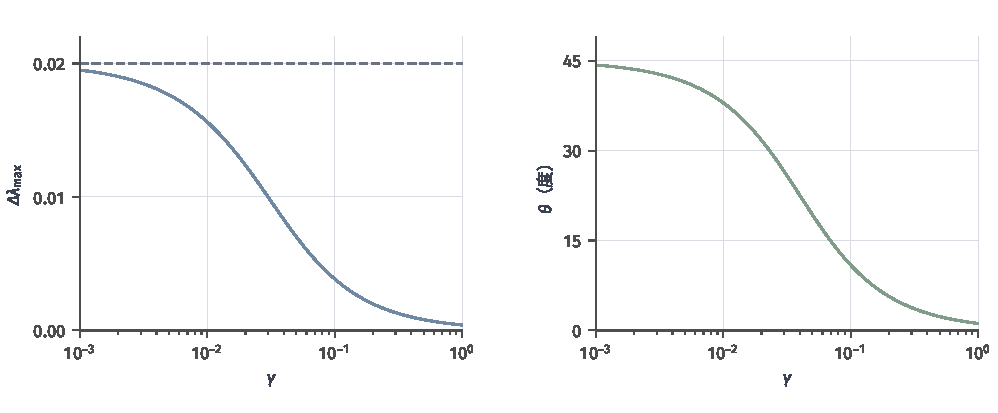
\includegraphics[width=0.92\linewidth]{figures/00-shared/mathematical-preliminaries-upper/02-linear-spaces/matplotlib/matrix-analysis-gap-direction/figure.pdf}
 \caption{谱隙与特征方向的转角（示例~\ref{ex:ls-gap-direction-rotation}，$t=0.02$）。横轴为原谱隙，
 图中记为$\gamma$，即正文的$\delta$。左：最大特征值的增量$r-\delta/2$，始终不超过虚线所示的$t$，
 符合Weyl界；右：最大特征方向的转角$\theta=\tfrac12\arctan(2t/\delta)$。谱隙远大于$t$时转角很小，
 谱隙小于$t$时转角接近$45^\circ$。}
 \label{fig:matrix-analysis-gap-direction}
\end{figure}

\paragraph{重根、奇异子空间与低秩近似}

谱隙只需存在于目标特征值组与组外之间，组内的特征值不必彼此分开。取$\bm S=\operatorname{diag}(2,2,0)$与$k=2$，原谱隙$\delta=2-0=2$。由上面的推论，$\lVert\bm E\rVert_2\leq\varepsilon<1$时，前二维特征子空间的最大主夹角满足$\sin\theta_{\max}\leq\varepsilon/(2-\varepsilon)<\varepsilon$，这个平面是稳定的。但平面内单个特征向量的选择并不稳定：取$\eta>0$，扰动$\eta\bm e_1\bm e_1^\top$使最大特征方向成为$\bm e_1$，扰动$\eta\bm e_2\bm e_2^\top$使它成为$\bm e_2$。无论$\eta$多小，两个结果都相互正交，而前二维子空间始终是$\operatorname{span}\{\bm e_1,\bm e_2\}$。所以不能把子空间内部基的变化解释为整个子空间发生了同样大的变化，反过来，子空间稳定也不保证其中每个基向量稳定。

奇异子空间可以通过对称增广矩阵回到特征子空间。设$\bm A,\bm E\in\mathbb R^{m\times n}$，$p=\min(m,n)$，$1\leq k<p$，前$k$个左、右奇异向量排成$\bm U_k$、$\bm V_k$。要求截断处的奇异值间隙$\delta_\sigma=\sigma_k(\bm A)-\sigma_{k+1}(\bm A)>0$，这也保证了所追踪的奇异值$\sigma_1,\ldots,\sigma_k$都为正。若$\sigma_k=0$，引理~\ref{lem:ls-symmetric-augmentation-spectrum}中的$\bm w_k^+$与$\bm w_k^-$对应同一个特征值$0$，就无法从增广矩阵的特征子空间中分出相应的奇异方向。由该引理，$\bm H(\bm A)$前$k$个特征值为$\sigma_1,\ldots,\sigma_k$，第$k+1$个为$\sigma_{k+1}$，对应的特征子空间由$\bm w_i^+$（$i\leq k$）张成，其正交投影为
\[
 \bm P_{\bm H}=\frac12\begin{bmatrix}\bm U_k\bm U_k^\top&\bm U_k\bm V_k^\top\\\bm V_k\bm U_k^\top&\bm V_k\bm V_k^\top\end{bmatrix}.
\]
设$\lVert\bm E\rVert_2\leq\varepsilon<\delta_\sigma/2$。由定理~\ref{thm:ls-weyl-singular-value}，$\bm A+\bm E$在截断处同样分开，对应的投影$\widetilde{\bm P}_{\bm H}$有相同的分块形式。$\bm H(\bm E)$的谱范数等于$\lVert\bm E\rVert_2$，对增广矩阵使用上面的推论，得$\lVert\bm P_{\bm H}-\widetilde{\bm P}_{\bm H}\rVert_2\leq\varepsilon/(\delta_\sigma-\varepsilon)$。矩阵左上块的谱范数不超过整个矩阵的谱范数（对单位向量$\bm x$，左上块乘$\bm x$是整个矩阵乘$(\bm x;\bm0)$所得向量的上半部分），而$\bm P_{\bm H}-\widetilde{\bm P}_{\bm H}$的左上块是$\tfrac12(\bm U_k\bm U_k^\top-\widetilde{\bm U}_k\widetilde{\bm U}_k^\top)$，所以
\[
 \lVert\bm U_k\bm U_k^\top-\widetilde{\bm U}_k\widetilde{\bm U}_k^\top\rVert_2\leq\frac{2\varepsilon}{\delta_\sigma-\varepsilon}\leq\frac{4\varepsilon}{\delta_\sigma},
\]
右下块给出右奇异子空间的同样结论。可见左、右奇异子空间的稳定性由截断处的间隙$\delta_\sigma$控制。

与上一小节对照：最佳秩$k$逼近的误差$\sigma_{k+1}$在任何情况下都只移动不超过$\varepsilon$，而取得这个误差所用的主方向只在截断处有足够间隙时才稳定。$\sigma_k=\sigma_{k+1}$时，最优误差仍然稳定，最优的秩$k$矩阵却可能在不同的子空间之间跳变。第~\ref{sec:ls-truncated-svd-ridge}节的截断求解直接用到这个区别：选取截断位置时，既要看被舍弃的奇异值是否可以忽略，也要看保留的方向是否与舍弃的方向分得开。

\subsection{一般方阵的谱敏感性}
\label{sec:ls-nonnormal-spectral-sensitivity}

前面按序比较特征值的界依靠对称结构：特征值是实数，可以排序，并由瑞利商刻画。一般方阵的特征值可能是复数，没有自然的次序，也没有瑞利商的极值表征。下面对可对角化的方阵研究另一个问题：$\bm A+\bm E$的某个特征值离$\bm A$的谱有多远。这里允许在复数域中选取特征基，向量使用复欧氏范数$\lVert\bm z\rVert_2=(\sum_i|z_i|^2)^{1/2}$，矩阵使用相应的诱导范数。

\begin{theorem}[Bauer--Fike]
\label{thm:ls-bauer-fike}
设$\bm A\in\mathbb C^{n\times n}$可对角化，$\bm A=\bm V\bm\Lambda\bm V^{-1}$，其中$\bm\Lambda=\operatorname{diag}(\lambda_1,\ldots,\lambda_n)$，$\bm V$可逆；记$\kappa_2(\bm V)=\lVert\bm V\rVert_2\lVert\bm V^{-1}\rVert_2$。则对任意$\bm E\in\mathbb C^{n\times n}$与$\bm A+\bm E$的任一特征值$\mu$，
\[
 \min_{1\leq i\leq n}|\mu-\lambda_i|\leq\kappa_2(\bm V)\lVert\bm E\rVert_2 .
\]
\end{theorem}
\begin{proof}
若$\mu$是$\bm A$的特征值，左端为零，结论成立。下设$\mu$不是$\bm A$的特征值，于是对角矩阵$\bm\Lambda-\mu\bm I$可逆。取$\bm A+\bm E$对应于$\mu$的特征向量$\bm w\neq\bm0$，由$(\bm A+\bm E)\bm w=\mu\bm w$得$(\bm A-\mu\bm I)\bm w=-\bm E\bm w$。代入$\bm A-\mu\bm I=\bm V(\bm\Lambda-\mu\bm I)\bm V^{-1}$，令$\bm y=\bm V^{-1}\bm w\neq\bm0$，得
\[
 \bm y=-(\bm\Lambda-\mu\bm I)^{-1}\bm V^{-1}\bm E\bm V\bm y .
\]
两边取范数，
\[
 \begin{aligned}
 \lVert\bm y\rVert_2
 &\leq\lVert(\bm\Lambda-\mu\bm I)^{-1}\rVert_2\,\lVert\bm V^{-1}\bm E\bm V\rVert_2\,\lVert\bm y\rVert_2\\
 &\leq\lVert(\bm\Lambda-\mu\bm I)^{-1}\rVert_2\,\kappa_2(\bm V)\lVert\bm E\rVert_2\,\lVert\bm y\rVert_2 .
 \end{aligned}
\]
对角矩阵$\bm D=\operatorname{diag}(d_i)$满足$\lVert\bm D\bm z\rVert_2^2=\sum_i|d_i|^2|z_i|^2\leq\max_i|d_i|^2\lVert\bm z\rVert_2^2$，且在相应的坐标向量处取等号，所以$\lVert(\bm\Lambda-\mu\bm I)^{-1}\rVert_2=1/\min_i|\lambda_i-\mu|$。代入并除以$\lVert\bm y\rVert_2>0$，得$1\leq\kappa_2(\bm V)\lVert\bm E\rVert_2/\min_i|\lambda_i-\mu|$，整理即得结论。
\end{proof}
界中出现的是所选特征基的条件数$\kappa_2(\bm V)$，而不是上一节的$\kappa_2(\bm A)$，二者衡量不同的东西。$\bm A=\operatorname{diag}(1,s)$（$0<s<1$）可取$\bm V=\bm I$，$\kappa_2(\bm V)=1$，任何扰动都只能使特征值移动不超过$\lVert\bm E\rVert_2$，而$\kappa_2(\bm A)=1/s$可以很大。反过来，取$\eta>0$与
\[
 \bm A=\begin{bmatrix}1&1\\0&1+\eta\end{bmatrix},\qquad
 \bm V=\begin{bmatrix}1&1\\0&\eta\end{bmatrix},
\]
由$\bm A(1,0)^\top=(1,0)^\top$与$\bm A(1,\eta)^\top=(1+\eta)(1,\eta)^\top$，$\bm V$的两列是特征值$1$与$1+\eta$的特征向量。$\eta\to0$时，$\bm A$趋于$\bm A_0=\left[\begin{smallmatrix}1&1\\0&1\end{smallmatrix}\right]$：$\bm A_0^\top\bm A_0=\left[\begin{smallmatrix}1&1\\1&2\end{smallmatrix}\right]$的特征值为$(3\pm\sqrt5)/2$，乘积为$1$，所以$\kappa_2(\bm A_0)=\sqrt{(3+\sqrt5)/(3-\sqrt5)}=(3+\sqrt5)/2\approx2.62$；又$\lVert\bm A-\bm A_0\rVert_2=\eta$，由定理~\ref{thm:ls-weyl-singular-value}，$\bm A$的两个奇异值与$\bm A_0$的相差不超过$\eta$，$\kappa_2(\bm A)$随之趋于$\kappa_2(\bm A_0)$，求逆并不敏感。但两个特征向量越来越接近平行：$\det(\bm V^\top\bm V)=(\det\bm V)^2$，所以$\bm V$的两个奇异值之积为$|\det\bm V|=\eta$，而最大奇异值不小于$\lVert\bm V\bm e_1\rVert_2=1$，故$\kappa_2(\bm V)\geq1/\eta$，Bauer--Fike界变得很宽。非正交的特征基会放大扰动在特征坐标中的表示，这是一般方阵特征值敏感的来源；对称矩阵可取正交的$\bm V$，$\kappa_2(\bm V)=1$，界与Weyl界同量级。

使用这个界时还要注意三点。第一，特征向量的缩放会改变$\bm V$的条件数，界对任意一组特征基成立，引用时须说明所用的基，通常取使$\kappa_2(\bm V)$较小的一组。第二，它只保证每个扰动后的特征值接近某个原特征值，不建立逐个特征值的固定配对，也不恢复对称情形的有序比较。第三，它要求$\bm A$可对角化；特征向量不足时，特征值的变化可以与扰动不成比例。
\begin{example}[特征值的移动远大于扰动]
\label{ex:ls-jordan-eigenvalue-sensitivity}
取不可对角化的
\[
 \bm A=\begin{bmatrix}0&1\\0&0\end{bmatrix},
\]
它的特征值全为$0$，特征空间只有一维。取扰动$\bm E=\left[\begin{smallmatrix}0&0\\t&0\end{smallmatrix}\right]$，$t>0$，则$\lVert\bm E\rVert_2=t$，而
\[
 \bm A+\bm E=\begin{bmatrix}0&1\\t&0\end{bmatrix},\qquad
 \det\bigl(z\bm I-(\bm A+\bm E)\bigr)=z^2-t ,
\]
特征值为$\pm\sqrt t$，移动量为$\sqrt t$。例如$t=10^{-10}$时特征值移动$10^{-5}$，是扰动大小的$10^5$倍。$\sqrt t/t\to\infty$（$t\to0^+$），所以不存在常数$c$使移动量对所有小扰动都不超过$c\lVert\bm E\rVert_2$。若改取$t<0$，特征值为$\pm\mathrm i\sqrt{|t|}$，实特征值随之消失。
\end{example}
这个例子说明，缺少可对角化条件时，特征值的变化可以出现与扰动不同的量级；本节不为此引入新的标准形体系。第~\ref{sec:multivariable-eigen-differential}节在相应光滑分支存在时研究一阶响应；本节的有限变化界则始终要连同对象的结构（对称、可对角化）和谱的分离条件一起使用。

综合起来，把矩阵本身当作输入时：对称矩阵的特征值与任意矩阵的奇异值都随扰动有界地移动，移动量不超过$\lVert\bm E\rVert_2$，并且不要求谱值分开，由此可以可靠地判断符号、正定性和秩的下界；所选子空间的方向要用主夹角比较，偏转由扰动与谱隙之比控制；一般方阵的特征值还取决于特征基的条件，甚至不与扰动成比例。条件数与谱的扰动讨论的都是一次作用或一次分解，下一节转向同一个矩阵的反复作用。
